%!TEX root = ../main.tex

\newpage

\chapter{Entwurf} %  (fold)
\label{cha:entwurf}

\section{Grober Entwurf (Architektur)}
\label{sec:grober_entwurf}

\section{Technologien}
\label{sec:technologien}

\section{Detaillierter Entwurf}
\label{sec:detaillierter_entwurf}

\subsection{GUI: Öffnung der App}
Die Öffnung der App resultiert erstmal darin die verfügbaren Cocktailmaschinen zu listen und den Nutzer wählen zu lassen. Ist die gewählte Cocktailmaschine kalibriert, wird der Nutzer sofort in das Menü versetzt. Ist die Maschine nicht kalibriert, wird der Nutzer in einen \hyperref[subsec:nocal]{Wartebereich} geschoben. Dort hat der Nutzer die Wahl:
\begin{itemize}
	\item den Kalibrierungstatus erneut abzufragen und bei positiver Bestätigung in dem Menü zu landen, 
	\item die Cocktailmachine zu wechseln
	\item oder die Cocktailmaschine zu kalibrieren.
\end{itemize}
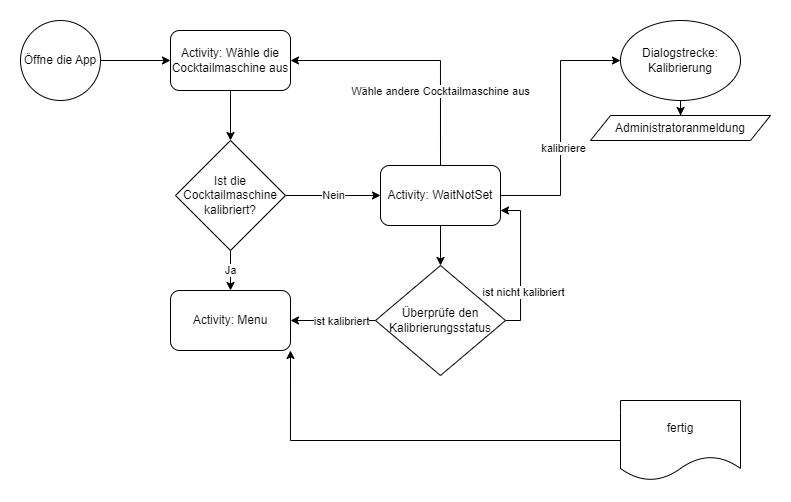
\includegraphics[scale=0.40]{Appstart.png}


\subsection{GUI: Keine Kalibrierung}
\label{subsec:nocal}

Drei mögliche Aktionen:

\begin{itemize}
\item anmelden
\item falsche Passwort: zurück in die Activity
\item und einleiten der automatischen Kalibrierung: Dialog: Kalibrierung
\item wähle eine andere Cocktailmachine aus: Cocktailmachinewahlactivity öffnet.
\item laden (Überprüfen, ob ein Admin die Kalibrierung vorgenommen hat)
\begin{itemize}

	\item Bei Erfolg (Admin hat die Kalibrierung getätigt. ): Hauptmenü öffnet
	
	\item Bei Misserfolg: Toast "Cocktailmaschine ist noch nicht bereit."

\end{itemize}
\end{itemize}


Nach der Auswahl eines der Möglichkeiten werden die Button auf nicht verfügbar gestellt, damit die Button beim Laden zwischen den Dialogen nicht angeklickt werden können.

\subsection{GUI: Dialog: Anmelden}

Dialogfenster:

Passwort angeben (''admin"). Gelange in den angemeldeten Zustand.

\subsection{GUI: Dialog: Automatische Kalibrierung}

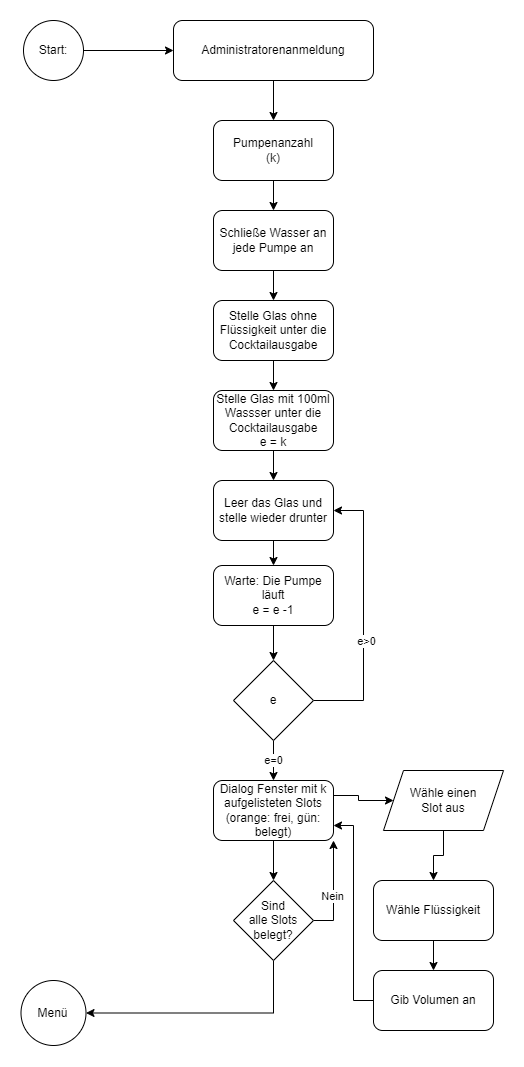
\includegraphics[scale=0.65]{calibrate.png}

\begin{enumerate}
\item Gebe die Anzahl (k) der Pumpen an.
\begin{enumerate}
	\item Toast ''Es lädt"	
\end{enumerate}
	\item Ok-Fenster: Schließe Wasser an die Pumpen.
	
	\item Ok-Fenster: Glas ohne Flüssigkeit
	
    \item Ok-Fenster: Glas mit 100ml Wassre
	
	\item Ok-Fenster: Leere das Glas
	
	\item Warte-Fenster: Pumpe läuft. k=k-1

\begin{enumerate}
		\item zu 5.: falls k>0
		
		\item zu 7.: sonst

\end{enumerate}
\item Dialog mit Liste von k Pumpen sind mit einer Slotnummer markiert und orange hinterlegt, wenn noch keine Flüssigkeit hinterlegt ist, und grün wenn eine Flüssigkeit hinterlegt ist.

\item Wähle orangene Pumpe.

\item Wähle Flüssigkeit.

\item Gibt Volumen an:
\begin{enumerate}

\item zu 7.: wenn noch nicht alle Flüssigkeiten ausgewählt wurden

\item zum Hauptmenü: sonst
\end{enumerate}
\end{enumerate}


\subsection{GUI: Darstellung Liste}
Liste von Elementen

Titel: Rezept, Zutaten, Serviervorschläge, Pumpen

Haus: Gehe zum Hauptmenü.

drehender Pfeil: Lade die Datenbank neu!

\subsubsection{Pumpen}

Statt dem Namen der Pumpen sind die Namen der zugeordneten Zutaten und die Slotnummer sichtbar.

\subsubsection{Rezepte}

Plus Zeichen: Gehe zur Erstellung eines Rezeptes.

\subsection{GUI: Anzeigen einzelner Elemente}

Für alle Elemente gilt: unter dem Titel ist ein Zeile mit drei Buttons. Der erste und linke Button ist ein Stift und öffnet die Änderungsseite für das Element. Der zweite und mittige Button ist ein drehender Pfeil. Er lädt die gesamte Datenbank neu und setzt die Seite neu auf. Der dritte und rechte Button ist eine Liste und öffnet die Liste der Elemente. Wird also eine Zutat angezeigt, so öffnet sich die Zutatenliste. Im weiteren wird von dieser Zeile als Menüzeile in der Einzelansicht gesprochen.

\subsubsection{Zutat}

Als Titel steht der Name der Zutat. Darunter kommt die Menüzeile. Unter der Menüzeile ist ein Gruppe von drei Sternen. Die Sterne haben die Farbe der Zutat. Darunter wird entweder angezeigt, dass die Zutat verfügbar oder nicht verfügbar ist. Dabei wird innerhalb einer Zeile links Ein grüner Punkt für verfügbar und dann neben der Text "verfügbar" angezeigt oder ein graues Kreuz und der Text "nicht verfügbar".

In der nächsten Zeile steht, ob die Zutat alkoholisch ist oder nicht. Dabei wird bei der Angabe alkoholisch eben der Text links angezeigt mit einem roten Warndreick auf der rechten Seite oder "nicht alkoholisch" mit einem grauen Warndreieck. Die Volumenanzeige gibt die Milliliterangabe an.

\subsubsection{Serviervorschlag}

Als Titel steht der Name des Serviervorschlags. Darunter ist die Menüzeile und da runter die Beschreibung.

\subsubsection{Pumpe}

Als Titel steht Slot und die Slotnummer. Die zugehörige Zutat wird angezeigt und das Volumen in Milliliter. Ein großer Button "Lass die Pumpe laufen".

\paragraph{Dialog: Pumpe laufen lassen}

Hier steht eine Aufforderung zur Milliliterangabe, um die Pumpe laufen zu lassen. Bei Bestätigung wird die Pumpe solange laufen gelassen.

\subsubsection{Rezepte}

Die Verfügbarkeitsanzeige ist ein grüner Punkt, wenn es verfügbar ist und rot, wenn es nicht verfügbar ist. Die Alkoholgehaltsanzeige ist ein Dreieck mit weißem Ausrufzeichen. Wenn das Dreieck rot ist, hat das Rezept alkoholische Zutaten. Wenn es grau ist, ist es nicht alkoholisch. Außerdem werden die Zutaten mit Milliliterangabe gelistet. Jede Zutat führt zur jeweiligen Zutatendarstellung. Die Serviervorschläge werden genauso gelistet. Zu letzt ist ein großer Button "Mix den Cocktail" fürt zu, Dialog: Mixen.

\paragraph{Dialog: Mixen/Activity:Simulation des Befüllens}

Beginnt mit einem CountDown mit der Anzahl der noch zu mixenden Cocktails bis zum eigenen Cocktail. Wenn der Nutzende dann dran ist, kommt die Aufforderung das eigene Glas runterzustellen, was bestätigt werden muss. Gehe zur Darstellung (Activity): Simulation des Befüllens, wenn das Mixen abgeschlossen ist, wird mit einem Dialog aufgefordert, den Cocktail abzuholen. Nach der Bestätigung des Abholens eird das Hauptmenü geöffnet.



\subsection{GUI: Ändern oder Hinzufügen}

Für alle Elemente gilt:

Möchte man ein neues Element hinzufügen. Geht man in die entsprechende Liste und wählt den Floatingbutton in der rechten unteren Ecke mit dem Plussymbol aus.

Jedes Element braucht einen Namen. Unter dem Titel gibt es ein Eingabefeld. Als Aufforderung steht in dem Feld in grauer Schrift "Füge einen Namen ein!". Wählt man das Feld aus, öffnet sich die Tastatur. Jetzt kann der Name eingegeben werden. Der eingegebene Name ist in schwarzer Schrift und nachdem ersten Einfügen eines Buchstabens ist die graue Aufforderung nicht mehr sichtbar. Handelt es sich hierbei allerdings um eine Änderung an einer bestehenden Element, dann ist zunächst die nich die Aufforderung zu sehen, sonder direkt der Name in schwarzer Schrift. Entfernt man alle Buchstaben in dem Feld, egal ob es sich um eine Änderung oder eine Neuerstellung handelt. Dann erscheint wieder die graue Aufforderung.

Unter all den Eingabefeldern. Stehen zwei Button "Abbruch" und "Speichern". Wählt man den Abbruch gelangt man in die Liste der Elementen. Wählt man den Speichervorgang. So wird die Detailansicht der neuerstellten Zutat sichtbar.

Der Speichervorgang wird abgebrochen, sollte beim Auslösen das Namensfeld leer sein.

\subsubsection{Zutat}

Daraufhin öffnet sich die AddAktivität. Der Titel heißt "Zutat".

Unter dem Namensfeld ist ein Switchbutton. Ist dieser aktiviert, steht direkt unter dem Button ein Feld "alkoholisch" mit einem roten Warndreieck davor. Ist der Button nicht aktitviert, ist das Warndreick grau und es steht "nicht alkoholisch" da. Bei der Neuerstellung ist zunächst der Switchbutton im nicht aktivenn Zustand und das Feld mit dem Warndreick ist nicht sichtbar. Erst nachdem der Nutzende mit dem Switchbutton interagierte wird die Warndreickzeile sichtbar. Bei der Änderung ist das Warndreick direkt sichtbar und der Switchbutton ist im aktiven oder inaktiven Zustand je nachdem ob die zu ändernde Zutat alkoholisch oder nicht ist.

Unter der Alkoholgehaltabfrage steht eine weitere Aufforderung "Ändere die Farbe!". Sie steht in einem Button. Wählt man diesen aus öffnet sich ein Dialog, in dem eine Farbe ausgewählt werden kann. Dieser Dialog kann abgebrochen werden mit "Abbruch". Mit dem "Speichern" wird der Zutat eine Farbe zu geordnet. Handelt es sich eine Neuerstellung und das erste Anklicken der Farbauswahl, so ist eine zufällige Farbe hinterlegt. Wurde bereits eine Farbe ausgewählt oder es ist eine Änderung, dann ist die derzeit zugeordnete Farbe der Ausgangspunkt. Der Button ändert seine Farbe mit der ausgewählten Farbe. Ist noch keine ausgewählt worden bei der Neuerstellung, so hat der Button die Standardbuttonfarbe.

\subsubsection{Serviervorschlag}

Als Titel steht "Serviervorschlag". Unter dem Namesfeld steht ein großes editierbares Textfeld. Dort steht in schwarz entweder die vorhandene Beschreibung bei einer Änderung oder in schwarz die eingegebene Beschreibung. Ist es eine Neuerstellung oder die gesamte Textfeldeingabe wurde entfernt (also die schwarzen Buchstaben), dann ist in grauen Buchstaben der Text "Füge eine Beschreibung ein." zu lesen, der so gleich wieder nicht sichtbar wird, sollte auch nur ein Buchstabe in diesem Feld eingegeben werden. Sind die Titelangabe oder die Beschreibungsangabe leer, dann wird das Speichern abgebrochen und eine Toastaufforderung zur Ergänzung angezeigt.

\subsubsection{Rezepte}

Unter dem Namensfeld steht für die Zutaten und die Serviervorschläge je eine Aufforderung des Einfügens mit einem grünen Plus daneben. Das Plus löst als Button einen Dialog aus, indem je entweder die Namen der verfügbaren Zutaten oder die der Serviervorschläge gelistet sind. Nach der Wahl einer Zutat wird in einem Dialog die Millilieterangabe gemacht und die Zutat mit Volumenangabe unter der Aufforderung hinzugelistet. Genauso sammeln sich die Namen der gewählten Serviervorschläge.

\subsubsection{Pumpe}

Es gibt kein Namensfeld. Es gibt zwei verpflichtende Felder: Ein Textfeld zur Angabe des Zutatennamens und der des Volumens. Beide müssen mit gültigen Werten ausgefüllt sein, um gespeichert zu werden.


\subsection{GUI: Menü}

Im Menü werden die wichtigsten Funktionen dem Nutzer angezeigt.

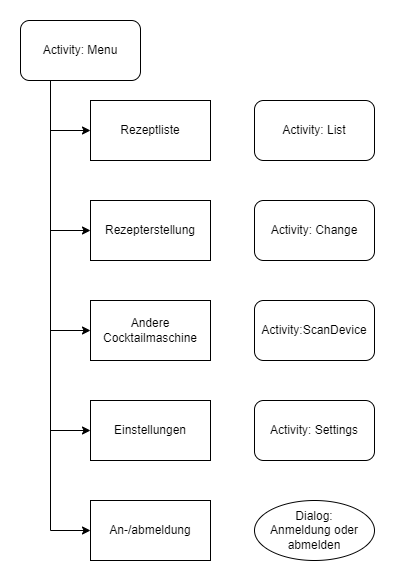
\includegraphics[scale=0.65]{Menu.png}
\captionof{figure}{Menü}
\newpage
\begin{sidewaystable}[]
	\centering
	\caption{Menü}
	
	\begin{tabular}{|l|l|l|l|l|l|}
		\hline
		Symbol  & Nächste Activity  & Funktion  & Sichtbar  & ausgelöste Reaktion \\ \hline
		Liste  & ListActivity  & Liste der Rezepte  & immer  & Aktivitätenwechsel \\ \hline
		Liste mit Plussymbol  & AddActivity  & Erstellung eines neuen Rezepts  & immer  & Aktivitätenwechsel \\ \hline
		Bluetooth mit Lupe  & BluetoothScanActivity  & Suche eine neue Cocktailmachine  & immer  & Aktivitätenwechsel \\ \hline
		Zahnrad  & Settingsactivity  & Einstellungsoptionen  & immer  & Aktivitätenwechsel \\ \hline
		Pfeil in eine Tür  & -  & Adminstratorenanmeldung  & Nur im abgemeldeten Zustand  & Zeigen eines Anmeldedialogs, Wechsel in den angemeldeten Zustand \\ \hline
		Pfeil aus einer Tür  & -  & Adminstratorenabmeldung  & Nur im angemeldeten Zustand  & Wechsel in den abgemeldeten Zustand \\ \hline
	\end{tabular}
	
\end{sidewaystable}


\subsection{GUI: Einstellung}

\subsubsection{Die Haupteinstellung:}
\begin{sidewaystable}[!ht]
	\centering
	\caption{Haupteinstellung}
	\begin{tabular}{|l|l|l|l|l|}
		\hline
		\textbf{Element } & \textbf{Nächste Activity } & \textbf{Funktion } & \textbf{Sichtbar } & \textbf{ausgelöste Reaktion} \\ \hline
		Anmelden  & -  & Adminstratorenanmeldung: Zeigen eines Anmeldedialogs, Wechsel in den angemeldeten Zustand  & Nur im abgemeldeten Zustand  & Funktion \\ \hline
		Abmelden  & -  & Adminstratorenabmeldung: Wechsel in den abgemeldeten Zustand  & Nur im angemeldeten Zustand  & Funktion \\ \hline
		Pumpe  & ListActivity  & Liste der Pumpen  & Nur im angemeldeten Zustand  & Aktivitätenwechsel \\ \hline
		Zutaten  & ListActivity  & Liste der verfügbaren Zutaten  & immer  & Aktivitätenwechsel \\ \hline
		Zutaten(Alle)  & ListActivity  & Liste der Zutaten  & Nur im angemeldeten Zustand  & Aktivitätenwechsel \\ \hline
		Rezepte  & ListActivity  & Liste der verfügbaren Rezepte  & immer  & Aktivitätenwechsel \\ \hline
		Rezepte(Alle)  & ListActivity  & Liste der Rezepte  & Nur im angemeldeten Zustand  & Aktivitätenwechsel \\ \hline
		Serviervorschläge  & ListActivity  & Liste der Serviervorschläge  & immer  & Aktivitätenwechsel \\ \hline
		Synchronisieren (Bluetooth)  & -  & Synchronisiere Rezpte und die Pumpen.  & immer  & Funktion \\ \hline
		Scannen (Bluetooth)  & ScanActivity  & Scanne nach der Cocktailmaschine  & immer  & Aktivitätenwechsel \\ \hline
		Cocktailmaschinen-einstellung  & MachineSettingsActivity  & weitere Einstellungen  & Nur im angemeldeten Zustand  & Aktivitätenwechsel \\ \hline
		Komplett neuladen (Datenbank)  & -  & Synchronisiere Pumpenstand und damit die Verfügbarkeit.  & immer  & Funktion \\ \hline
		Füge vorbereitete Rezepte hinzu (Datenbank)  & -  & Lade Rezepte aus Json und CSV-Dateien.  & immer  & Funktion \\ \hline
	\end{tabular}
\end{sidewaystable}

\subsubsection{Die Cocktailmaschineneinstellungen:}
(Erreichbar nur im \textbf{an}gemeldeten Zustand)

\begin{sidewaystable}[!ht]
	\centering
	\caption{Cocktailmaschineneinstellungen}
	\begin{tabular}{|l|l|l|l|}
		\hline
		\textbf{Element } & \textbf{Nächste Activity } & \textbf{Funktion } & \textbf{ausgelöste Reaktion} \\ \hline
		Neukalibrierung (Kalibrierung)  & WaitNotSet  & Setze die Kalibrierung zurück und kalibriere die Cocktailmaschine neu. Geh zu WaitNotSet.  & Aktivitätenwechsel \\ \hline
		Waagenkalibrierung (Kalibrierung)  & ScaleSettingsActivity  & weitere Einstellungen  & Aktivitätenwechsel \\ \hline
		Pumpenkalibrierung (Kalibrierung)  & PumpSettingsActivity  & weitere Einstellungen  & Aktivitätenwechsel \\ \hline
		Statusabfrage (Zustand)  & -  & Zeige in einem Dialog den derzeitigen Zustand an, wie von Feya beschrieben.  & Funktion \\ \hline
		Reinigung (Zustand)  & -  & Schickt Reinigungsbefehl  & Funktion \\ \hline
		Neustart (Neustart)  & -  & Schickt Neustartbefehl. (Kein Zurücksetzen!)  & Funktion \\ \hline
		Werkseinstellungen (Neustart)  & WaitNotSet  & Setze die Kalibrierung zurück. Geh zu WaitNotSet.  & Aktivitätenwechsel \\ \hline
	\end{tabular}
\end{sidewaystable}



\subsubsection{Die Waagenkalibrierung:}
(Erreichbar nur im \textbf{an}gemeldeten Zustand)
\begin{sidewaystable}[!ht]
	\centering
	\begin{tabular}{|l|l|l|l|}
		\hline
		\textbf{Element } & \textbf{Nächste Activity } & \textbf{Funktion } & \textbf{ausgelöste Reaktion} \\ \hline
		Kalibriere  & -  & Setze das Gewicht mit Hilfe eines Dialogs. Schicke Gewichtsangabe.  & Funktion \\ \hline
		Tariere  & -  & Schicke Tarierungsbefehl.  & Funktion \\ \hline
		Skaliere  & -  & Setze Saklierungsfaktor mit des Dialogs.  & Funktion \\ \hline
		derzeitges Gewicht  & -  & Zeige in einem Dialog den derzeitiges Gewicht an.  & Funktion \\ \hline
	\end{tabular}
\end{sidewaystable}

\subsubsection{Die Pumpenkalibrierung:}
(Erreichbar nur im \textbf{an}gemeldeten Zustand)
\begin{sidewaystable}[!ht]
	\centering
	\begin{tabular}{|l|l|l|l|}
		\hline
		\textbf{Element } & \textbf{Nächste Activity } & \textbf{Funktion } & \textbf{ausgelöste Reaktion} \\ \hline
		Automatische Kalibrierung  & WaitNotSet  & Setze die Kalibrierung zurück und kalibriere die Cocktailmaschine neu. Geh zu WaitNotSet.  & Aktivitätenwechsel \\ \hline
		Setze Pumpzeiten (Kalibrierung)  & -  & Dialog mit vier Eingabefeldern: Zeit1, Zeit2, Volumen1, Volumen2, wie von Freya beschrieben. Wird für alle Pumpen gleichzeitig verwendet.  & Funktion \\ \hline
	\end{tabular}
\end{sidewaystable}




\subsection{Datenbank}

